\chapter{Resultados}
%Conforme afirmado por Jeffrey L. Overbey e Ralph E. Johnson em ~\cite{Overbey:2009}, Java mantém construções ultrapassas ao longo das versões do desenvolvimento do software o que de fato acontece devido a compatibilidade mantida entre as versões da linguagem. Tais construções somente seriam evitadas caso ocorresse um grande e radical \textit{refactoring} como ocorreu na linguagem Fortan~\cite{Overbey:2009}, quando foi introduzido o paradigma de orientação a objeto que acarretou na quebra de compatibilidade com a versões anteriores.
%
%Baseado nesta assertiva este trabalho tem como principal objetivo de encontrar construções obsoletas e encontrar possíveis casos de trechos de código que poderiam ter sido evoluídos ao longo das versões de Java e que não evoluíram. Neste caso esta sendo pesquisado caso onde deveriam ter sofrido o \textit{refactoring} baseado nas características de Java 7 e Java 8. Dentre as característica mais importante a ser procuradas estão:
%
%\begin{itemize}
%\item Adoção e oportunidades de Multicatch.
%\item Adoção de Try com resource.
%\item Adoção e oportunidades de Switch com String.
%\item Adoção de Expressões Lambda.
%\item Oportunidades de exist - Expressões Lambda.
%\item Oportunidades de filter - Expressões Lambda.
%\item Oportunidades de map - Expressões Lambda.
%\end{itemize}
%
%Além da replicação do estudo de Parnin .et.al~\cite{Parnin:ACM2011} e diferentemente do trabalho original, estender  como objetivo compreender como a adoção de Generics se correlaciona com a data de lançamento inicial dos
%projetos selecionados. 

Para a realização deste trabalho foram escolhidos 47 projetos open-source separados em 3 grupos \textbf{G1} projetos iniciados antes do lançamento de \textit{Generics}, \textbf{G2} projetos iniciados após o lançamento de \textit{Generics} e \textbf{G3} projetos com a última \textit{release} em 2015. Alguns destes projetos são os mesmos utilizados em, \cite{Parnin:ACM2011, Dyer:ACM2014, ward2015performance}, este também fora separados pela natureza da aplicação,  Aplicações, Bibliotecas e Servidores/Banco de dados conforme tabela:~\ref{tab:systems} o que totalizou mais de 8.5M de~\acs{LOC}.

%Os dados contidos no arquivos ~\acs{CSV} foram processados e analisados com o software R~\cite{R} versão (3.1.2) além da biblioteca ggplot~\cite{ggplot} versão (1.0.1) para gerar gráficos mais consistentes.

\begin{table}[h]\footnotesize
\centering
	\caption{Projetos.}
	\begin{tabular}{l|lccrr}\hline
		 & \textbf{System} & \textbf{Release} & \textbf{Group}  & \textbf{LOC} \\\hline \hline
		\multirow{22}{*}{\rotatebox[origin=c]{90}{\textbf{Application}}} 
																 & ANT & 1.9.6 & G1 & 135741\\
																 & ANTLR  & 4.5.1 & G1/G3 & 89935 \\
																 & Archiva  & 2.2.0 & G2/G3 & 84632\\
																 & Eclipse & R4\_5 & G1 & 13429\\
																 & Eclipse-CS & 6.9.0 & G1 & 20426\\
																 & FindBugs & 3.0.1 & G1/G3 & 131351\\
																 & FitNesse & 20150814 & G2/G3 & 72836\\
																 & Free-Mind & 1.0.1 & G1 & 67357\\
																 & Gradle & 2.7 & G2 & 193428\\
																 & GWT & 2.7.0 & G2 & 15421\\
																 & Ivy & 2.4.0 & G2/G3 & 72630\\
																 & jEdit & 5.2.0 & G1 & 118492\\
						   									     & Jenkins & 1.629 & G2/G3 & 113763\\
																 & JMeter & 2.13 & G1/G3 & 111317\\
																 & Maven & 3.3.3 & G1/G3 & 78476\\
																 & Openmeetings & 3.0.6 & G2/G3 & 50496\\
																 & Postgree JDBC & 9.4.1202 & G1/G3 & 43596\\ 
																 & Sonar & 5.0.1 & G2/G3 & 362284\\
																 & Squirrel & 3.4.0 & G1 & 252997\\
																 & Vuze & 5621-39 & G1 & 608670\\
																 & Weka & 3.6.12 & G1 & 274978\\
																 \hline
					
					\multirow{18}{*}{\rotatebox[origin=c]{90}{\textbf{Library}}} 
																  & Axis & 1.4 & G2 & 121820\\		
																  & Commons Collections & 4.4.0 & G1 & 51622\\
																  & Crawler4j & 4.1 & G2/G3 & 3986\\
																  & Hibernate & 5.0.1 & G1/G3 & 541116\\
																  & Isis & 1.9.0 & G2 & 262247\\
																  & JClouds & 1.9.1 & G2/G3 & 301592\\
																  & JUnit & 4.1.2 & G1/G3 & 26456\\
																  & Log4j & 2.2 & G1/G3 & 69525\\
   						   									      & MyFaces & 2.2.8 & G2/G3 & 222865& \\
																  & Quartz & 2.2.1 & G2 & 31968\\
																  & Spark & 1.5.0 & G2/G3 & 31282\\
																  & Spring-Framework & 4.2.1 & G1/G3 & 531757\\
																  & Storm & 0.10.0 & G2/G3 & 98344\\
															      & UimaDucc & 2.0.0 & G2 & 96020\\
																  & Wicket & 7.0.0 & G2/G3 & 211618\\
																  & Woden & 1.0 & G2/G3 & 29348\\
																  & Xerces & 2.11.0 & G1 & 126228\\	
																  \hline		
																					 
					\multirow{8}{*}{\rotatebox[origin=c]{90}{\textbf{Servers - Databases}}} 
																  & Cassandra & 2.2.1 & G2/G3 & 282336\\	
																  & Hadoop & 2.6.1 & G2/G3 & 896615\\
						   									      & Jetty & 9.3.2 & G1 & 299923\\
																  & Lucene & 5.3.1 & G1 & 506711\\
						   									      & Tomcat & 8.0.26 & G1/G3 & 287897\\
						   									      & UniversalMedia Server & 5.2.2 & G3 & 54912\\
						   									      & Wildfly & 9.0.1 & G1/G3 & 392776\\ 
						   									      & Zookeeper & 3.4.6 & G3 & 61708\\ 
						   									      \hline		

	\label{tab:systems}
	\end{tabular}
\end{table}




\section{Generics}
Relacionado com a adoção de \textit{Generics}, foi descoberto que o maioria dos projetos apresentam um porção significante entre a quantidade de tipos genéricos e a quantidade total de tipos declarados em média(5.31\% e 12.31\%). Pode-se comprovar que em 16\% dos sistemas não declaram nenhum tipo genérico e que o projeto \textit{Commons Collections} é o sistema que com a relação mais expressiva de tipos parametrizados: 75\% de todos os tipos declarados são genéricos.

Também foi investigado a relação entre tipos genéricos declarados e todos os tipos considerando o tipo e idade do sistemas. Tabela:~\ref{tab:std} apresenta um resumo desta observação onde é possível comprovar que o uso típico de Java \textit{Generics} não muda significativamente entre os tipos de projetos Java, embora essa proporção seja mais baixa para Aplicações e servidores/bancos de dados com versões anteriores ao lançamento do Java SE 5.0.

\begin{table}[h]
	\centering
	\caption{Resumo dos tipos agrupados por idade e do tipo dos projetos.}
	\begin{tabular}{ccccc} \hline 
		Tipo de Projeto & Antes Java SE 5.0 & Tipo & Tipo Genérico & Ratio(\%) \\ \hline\hline
		Aplication & Yes & 18168 & 177 & 0.99 \\
		Aplication & No & 16148 & 744 & 5.39 \\
		Library & Yes & 21537 & 1198 & 5.26 \\
		Library & No & 22639 & 947 & 4.36 \\
		Server/Database & Yes & 18038 & 552 & 2.97 \\ 
		Server/Database & No & 11790 & 760 & 6.06 \\ \hline
	\end{tabular}
	\label{tab:std} %std means summary of type declarations
\end{table}


Há também um número expressivo de campos e variáveis declaradas como instâncias de tipos genéricos. Isto é, a partir de 925925 variáveis e campos declarados em todos os projetos, 84.880 são instâncias de tipos genéricos, 10 \% de todos os campos e variáveis declaradas. Além disso, a partir destes campos e as variáveis declaradas como instância de tipos genéricos, quase 17\% são instâncias dos tipos presentes na Tabela:~\ref{tab:tipoXnumeroInstancia}. Note que, em um trabalho anterior, Parning et al.~\cite{Parnin:ACM2011} apresenta \texttt{List$<$String$>$} com quase 25\% de todos os genéricos. Aqui pode ser confirmado que \texttt{List$<$String$>$} ainda é o tipo mais frequente na ocorrência de tipos genéricos, embora não tão difundido anteriormente. No entanto com 730720 métodos, apenas entre 6157, 0.84\%, são \emph{métodos parametrizados.}

\begin{table}[ht]
	\centering
	\caption{Tipo declarado X Número de instancia}
	\begin{tabular}{cc}
		\hline
		Tipo & Número de Instância\\ 
		\hline \hline
		\texttt{List$<$String$>$} & 4993 \\ 
		\texttt{Class$<$?$>$} & 3033 \\ 
		\texttt{Set$<$String$>$} & 2872 \\ 
		\texttt{Map$<$String,String$>$} & 2294 \\ 
		\texttt{Map$ < $String,Object$>$} & 1554 \\ \hline
	\end{tabular}
	\label{tab:tipoXnumeroInstancia} %std means summary of type declarations
\end{table}

Também fora investigado o uso mais avançado de Java \textit{Generics}, incluindo construções que fazem polimorfismo parametrizado. Com este recurso é possível criar classes paramétricas que aceitam qualquer tipo \textbf{T} como argumento, uma vez que um tipo \textbf{T} satisfaça um determinada pré-condição isto é, o tipo \textbf{T} deve ser um qualquer um subtipo (usando o modificador \textit{extends}) ou um super-tipo ( usando o modificador \textit{super}) de um determinado tipo existente. Estes modificadores pode ser usado tanto na declaração de novos tipos, bem como na declaração de campos e variáveis em combinação com o wildcard \textbf{?}). A partir de 4355 tipos genéricos declarados em todos os sistemas, descobriu-se que 1.271, quase 30\% usam alguns desses modificadores, extends, super, ou ?. Notavelmente, o modificador \textit{extends} é o mais comum, e está presente em todos os tipos genéricos que usam os modificadores \textit{?} e \textit{super}. Em alguns casos de uso são combinações de modificadores, como no exemplo da Listing:~\ref{lst:tp}, onde a classe IntervalTree (projeto CASSANDRA) é parametrizado de acordo com três parâmetros de tipo (C, D e I). Com relação aos campos e declarações de variáveis, quase 13\% de todos os casos genéricos usam o \textit{?} \textit{wildcard} e 3,13\% usam o \textit{extends}.

\begin{lstlisting}[caption={Declaração não trivial de Generics.}\label{lst:tp},language=Java] 
public class IntervalTree<C extends Comparable<? super C>, D, I extends Interval<C, D>> implements Iterable<I>{
  //...
}
\end{lstlisting}


Em suma, os resultados mostram que Java \textit{Generics} é uma \textit{feature} em que corresponde a 5\% de todos os tipos declarados dos sistemas, portanto, um grande quantidade de código repetido e tipo coerções (moldes) foram evitado usando tipos genéricos. Além disso, a partir desses tipos genéricos, quase 30\% usam um recurso avançado (como amplia e de super envolvendo parâmetros de tipo). Também foi descoberto que quase 10\% de todos os atributos e variáveis declaradas são tipos genéricos, embora a maior parte são instâncias de tipos genéricos da biblioteca \textit{Java Collection}. Finalmente, embora Parnin et ai.~\cite{Parnin:ACM2011} argumentam que uma classe como \textit{StringList} pode cumprir 25\% das necessidades de desenvolvedores entretanto, o uso de Java \textit{Generics}  não deve ser negligenciada devido aos benefícios que são incorporados ao sistema.



\section{Lambda Expression}
Considerando os sistemas, foi encontrado um uso limitado de Expressões Lambda- independentemente das expectativas e reivindicações sobre os possíveis benefícios dessa construção. Na verdade, apenas cinco projetos faz a adoção deste recurso conforme a Tabela:~\ref{tab:adocaoLambda}, embora a maioria dos cenários de uso (quase 90\%) estão relacionados com testes de unidade. Em um primeiro momento, este resultado nos levou a pensar que alguma nova versão de um quadro de teste de unidade poderia ter sido orientador develpers para testar o uso de expressões lambda. No entanto, depois de analisar manualmente o código-fonte, não encontramos qualquer orientação como essa ea adoção de expressões lambda para teste deve ocorrer de forma ad-hoc (como esforços individuais). Ou seja, a partir de milhares de casos de teste de unidade em Hibernate, a poucos testes para uma biblioteca específica (relacionados com cache) usar expressões lambda. Este pequeno uso de expressões lambda pode ser principalmente justfied por uma decisão estratégica de projetos estabelecidos para evitar a migração anterior do código-fonte para novas versões de um idioma.

\begin{table}[h]
	\centering
	\caption{Ocorrências de Expressões Lambda.}
	\begin{tabular}{cc}
		\hline
		Sistema & Ocorrências Expressões Lambda\\ 
		\hline \hline
		\texttt{Hinernate} & 168 \\ 
		\texttt{Jetty} & 2 \\ 
		\texttt{Lucene} & 11 \\ 
		\texttt{Spark} & 77 \\ 
		\texttt{Spring-framework} & 121 \\ \hline
	\end{tabular}
	\label{tab:adocaoLambda} %std means summary of type declarations
\end{table}


Foi enviado mensagens para grupos do desenvolvedores sobre o assunto, e algumas respostas esclarecem a atual situação da adoção de Expressões Lamdba. Primeiro de tudo, para os sistemas estabelecidos, as equipes de desenvolvedores muitas vezes não podem assumir que todos os potenciais utilizadores são capazes de migrar para uma nova versão do \textit{Java Runtime Environment}. Por exemplo, o seguinte \textit{post} explica uma das razões para um determinado projeto não adotar algumas construções de linguagem Java: "É, sobretudo, para permitir que as pessoas que estão vinculados (por qualquer motivo) para versões mais antigas do ~\acs{JDK} para usar nosso software. Há um grande número de projetos que não são capazes de usar novas versões do ~\acs{JDK}. Eu sei que este é um tema controverso e acho que a maioria de gostaria de usar todos esses recursos. Mas não devemos esquecer as pessoas usando nosso software em seu trabalho diário" (http://goo.gl/h0uloY).

Além disso, um abordagem inicial utilizando uma nova característica da linguagem é mais oportunista. Ou seja, os desenvolvedores não migram todo o projeto, mas em vez disso as modificações para introduzir novas construções de linguagem ocorrem quando eles estão implementando novas funcionalidades. Duas respostas a estas perguntas deixam isso claro: "Nós tentamos evitar reescrever grandes trechos de código base, sem uma boa razão. Em vez disso, tirar proveito dos novos recursos de linguagem ao escrever novo código ou refatoração código antigo."(https://goo.gl/2WgjVG) e "Eu, pessoalmente, não gosto da ideia de mover todo o código para uma nova versão Java, eu modifico áreas que atualmente trabalho."(http://goo.gl/ GQ4Ckn). Observe que não se pode generalizar estas conclusões com base nessas respostas, uma vez que não realizar um inquérito mais estruturado. No entanto, estas respostas podem apoiar trabalhos contra a adoção antecipada de novos recursos de linguagem por sistemas estabelecidos com uma enorme comunidade de usuários.


Também foi efetuada uma busca no STACK OVERFLOW tentando descobrir se expressões lambda é um tema discutido atualmente ou não~\footnote{Última pesquisa realizada em Novembro 2015}, utilizando \textit{tags} Java e Lambda. Foi encontrada mais de 1000 questões respondidas. Este número é bastante expressivo, quando considerou-se uma busca por questões marcadas com as \textit{tag} de Java Generics levou-se a um número próximo de 10 000 perguntas, embora \textit{Generics} tenha sido introduzido há mais de dez anos. Possivelmente, expressões lambda está sendo usado principalmente em pequenos projetos e projetos experimentais. Isso pode contrastar com os resultados de ~\cite{Dyer:ACM2014}, que sugerem uma adoção antecipada de novos recursos da linguagem (mesmo antes de lançamentos oficiais da característica). Com base nesses resultados, pode-se comprovar com este trabalho que a adoção antecipada de novos recursos da linguagem ocorre em projetos pequenos e projetos experimentais.

Outra investigação foi se existia a oportunidade de adoção de Expressões Lambda nos projetos estudados. Desta forma, foi complementado um testou maior~\cite{gyori2013crossing},  que investigou as mesmas questões porém eu um número de  inferior de projetos. Existem dois cenários típicos para \textit{refactoring} utilizando Expressões Lambda: \textit{Annonymous Inner Classes} (~\acs{AIC}) e \textit{Enhanced for Loops} (~\acs{EFL}). É importante notar que nem todas as ~\acs{AIC}s e ~\acs{EFL}s podem ser reescritas utilizando Expressões Lambda, e existem rígidas precondições que são detalhadas em ~\cite{gyori2013crossing}. Neste trabalho foi utilizado uma abordagem mais conservadora para considerar se é possível refatorar ~\acl{EFL} para Expressão Lambda para evitar falsos positivos.  Entretanto, foi considerado somente oportunidades de refatorar ~\acs{EFL} para Expressões Lambda em 3 particular casos: EXIST PATTERN, BASIC FILTER PATTERN e BASIC MAPPING PATTERN de acordo com os Listing:~\ref{lst:exist},~\ref{lst:filter} e~\ref{lst:map}.

\begin{lstlisting}[caption={EXIST PATTERN.}\label{lst:exist},language=Java]
//...
for(T e : collection){
	if(e.pred(args)){
		return true;
	}
}
return false;

//pode ser refatorado para:
return collection.stream().anyMatch(e->pred(args));
\end{lstlisting}

\begin{lstlisting}[caption={FILTER PATTERN.}\label{lst:filter},language=Java] 
//...
for(T e : collection){
	if(e.pred(args)){
		otherCollection.add(e);
	}
}

//pode ser refatorado para:
collection.stream().filter(
		e->pred(args).forEach(e->otherCollection.add(e)
	);
\end{lstlisting}

\begin{lstlisting}[caption={MAP PATTERN.}\label{lst:map},language=Java] 
//...
for(T e : collection){
	e.foo();
	e = blah();
	otherCollection.add(e);
}

//pode ser refatorado para:

collection.stream().forEach(e->{
	e.foo();
	e = blah();
	otherCollection.add(e);
});
\end{lstlisting}

Mesmo com um abordagem conservador, foi encontrada 2496 casos em que poderia ser efetuado \textit{refactoring} ~\acs{EFL} para Expressão Lambda. Atualmente, a maior parte destes casos 2190 correspondem ao MAP PATTERN.


Também foi investigado o típico uso de características de concorrência em Java. Foi encontrado que 39 de 43 dos sistemas declarados classes que herdam de \textit{Thread} ou implementam a interface \textit{Runnable}. A Tabela:~\ref{tab:concorrenciaJava} apresenta a relação destas declarações quando considerado o número total de tipos declarados, agrupados projetos estudados. Note que o uso de classes que herdam de \textit{Thread} ou implementam \textit{Runnable} é elevado considerando os casos de servidores e database.

\begin{table}[h]
	\centering
	\caption{Classes concorrentes que \textit{extends Thread} ou implementam \textit{Runnable}.}
	\begin{tabular}{cc}
		\hline
		Tipo Sistema & Relação dos Tipos de Concorrência\\ 
		\hline \hline
		\texttt{Applications} & 0.69 \\ 
		\texttt{Libraries} & 0.34 \\ 
		\texttt{Serves and database} & 1.52 \\ \hline
	\end{tabular}
	\label{tab:concorrenciaJava} %std means summary of type declarations
\end{table}

%\section{Lambda}
Ao todo o visitor responsável por pesquisar a adoção de \textit{Lambda} encontrou somente 814 caso de uso. Distribuidos em 354 arquivos o que leva a acreditar que tal característica não esta sendo tão relevante quanto sua espectativa de lançamento. Onde somente 2 casos não estão envolvidos em testes unitátos, os demais 812 estão sendo empregados no desevolvimento de testes unitários conforme exibido pela figura: \ref{fig:AdocaoLambda}. Vale resaltar que somente duas únicas ocorrências de lambda foram encontradas no projeto Jetty versão 9.3.2 nos fontes \textit{PathMap.java} e \textit{RegexSet.java}.\\

\begin{figure}[h]
	\center
	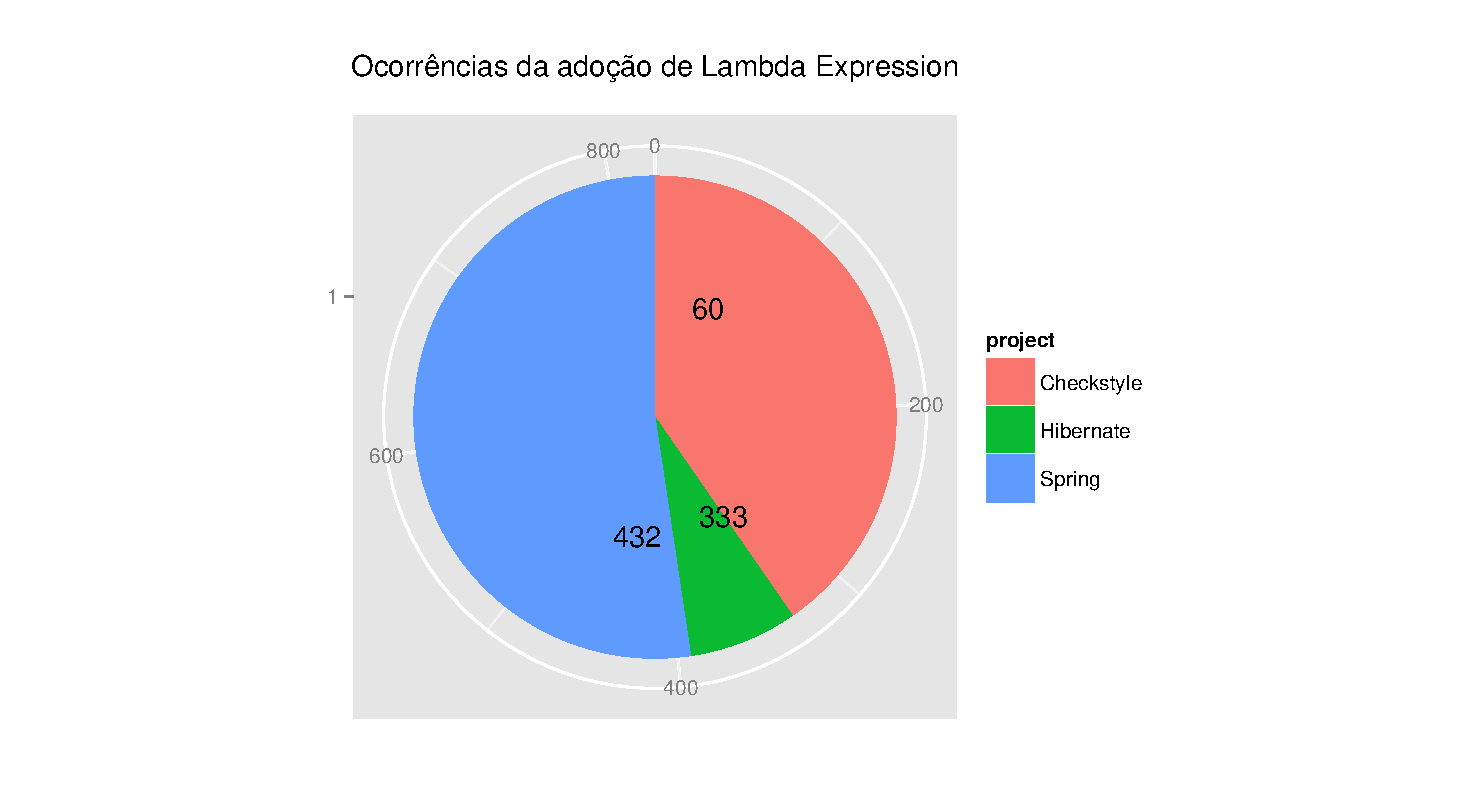
\includegraphics[scale=0.8]{Imagens/AdocaoLambdaTestes}
	\label{fig:AdocaoLambda}
	\caption{Adoção de \textit{Lambda} em testes unitários.}
\end{figure}



\subsection{Oportunidades de Aplicar Lambda}
Entretanto foram encontradas XXXXX oportunidades de converter \textit{For} que iteram \textit{Collections} para \textit{Lambda} através da \textit{Inteface Stream}, totalizando XXX \acs{LOC}. Estas esão dividida confome a figura: \ref{OpportunidadesLambda}.\\

%\subsection{Oportunidades para uso da constru\c c\~{a}o \texttt{multi-catch}}

O uso da constru\c c\~{a}o \texttt{multi-catch} permite reduzir qualquer 
l\'{o}gica duplicada existente em blocos \texttt{catch} distintos de 
uma contru\c c\~{a}o \texttt{try-catch}. Com as an\'{a}lises realizadas, 
foi poss\'{i}vel identificar uma quantidade significativa de oportunidades 
de uso dessa constru\c c\~{a}o, conforme exibido na Figura: \ref{fig:Muticatch}. Ao todo, 
foram encotrados \num{10368} blocos \texttt{try} que possuem \textit{catchs} repetidos. 
Essas ocorrências estão distribuídas em \num{7297} arquivos e totalizamo \num{97347} \acs{LOC}. 
Importante observar que o teste de  similaridade entre os blocos \texttt{catch} 
foi realizado através de uma chamada a um método exteno que verificava a igualdade da \'{a}rvore 
sint\'{a}tica. Apesar dessa abordagem n\~{a}o fazer uso de uma estrat\'{e}gia de an\'{a}lise 
de similaridade de c\'{o}digo mais robusta, a mesma pode ser facilmente alterada de 
acordo com algum algoritmo existente. 


\begin{figure}[h]
	\center
	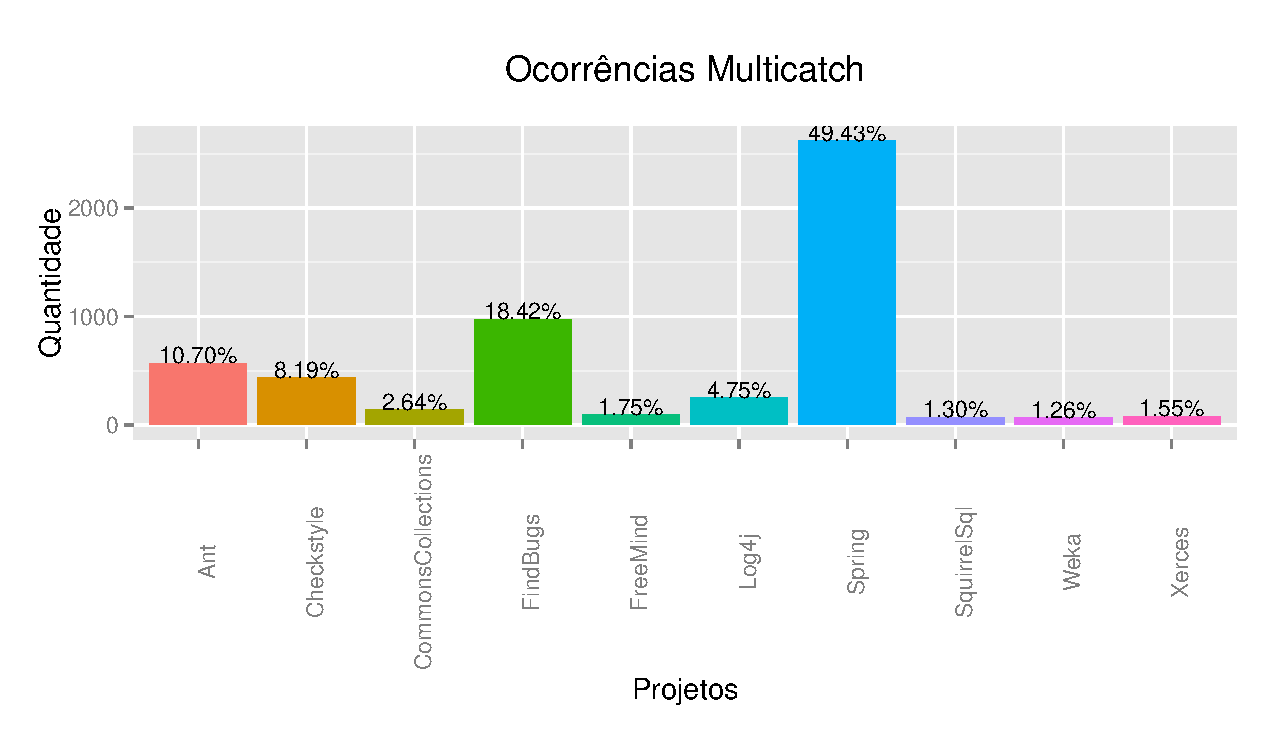
\includegraphics[width=13cm,height=7.8cm]{Imagens/ocorrenciasMulticatch}
	\label{fig:Muticatch}
	\caption{Oportunidades de \textit{Multicatch} nos projetos.}
\end{figure}
		

Considere os exemplos nas listagens {\color{red} X e Y}, 
encontrados na classe \texttt{AbstractNestablePropertyAccessor} do projeto \textit{Spring 4.2.0.RC2}. 
Neste caso, é possível reestruturar o c\'{o}digo para usar a constru\c c\~{a}o 
\texttt{multi-catch}, o que levaria a uma redu\c c\~{a}o de {\color{red} 40\%}  para 
esse trecho de código. Um simples \textit{refactoring} unindo todos os blocos 
que potencialmente se beneficiariam do uso de blocos \texttt{multi-catch} levaria a uma redução de 
68063 \acs{LOC}, tornando essa constru\c c\~{a}o  \'{u}til para reduzir a quantidade de 
linhas de c\'{o}digo em duplicidade de um projeto. 
\begin{lstlisting}[]
// Sem uso de Multicacth 17 LOC
try {...}
catch (ConverterNotFoundException ex) {
  PropertyChangeEvent pce = new PropertyChangeEvent(this.rootObject, this.nestedPath + propertyName, oldValue, newValue);
  throw new ConversionNotSupportedException(pce, td.getType(), ex);
}catch (ConversionException ex) {
  PropertyChangeEvent pce = new PropertyChangeEvent(this.rootObject, this.nestedPath + propertyName, oldValue, newValue);
  throw new TypeMismatchException(pce, requiredType, ex);
}catch (IllegalStateException ex) {
  PropertyChangeEvent pce = new PropertyChangeEvent(this.rootObject, this.nestedPath + propertyName, oldValue, newValue);
  throw new ConversionNotSupportedException(pce, requiredType, ex);
}catch (IllegalArgumentException ex) {
  PropertyChangeEvent pce = new PropertyChangeEvent(this.rootObject, this.nestedPath + propertyName, oldValue, newValue);
  throw new TypeMismatchException(pce, requiredType, ex);
}
\end{lstlisting}


\begin{lstlisting}
 //  Com uso de Multicatch 10 LOC
 try {...}
 catch (ConverterNotFoundException ex | IllegalStateException ex) {
   PropertyChangeEvent pce = new PropertyChangeEvent(this.rootObject, this.nestedPath + propertyName, oldValue, newValue);
   throw new ConversionNotSupportedException(pce, td.getType(), ex);
 }catch (ConversionException ex | IllegalArgumentException ex) {
   PropertyChangeEvent pce = new PropertyChangeEvent(this.rootObject, this.nestedPath + propertyName, oldValue, newValue);
   throw new TypeMismatchException(pce, requiredType, ex);
 }	
\end{lstlisting}

%Uma análise mais detalhada sobre \textit{JBoss, Spring, Hibernate e Findbugs} totalizando juntos 7778 ocorrências, iniciando na 3.0.0.M1 lançada em junho de 2009 até a mais recente até o momento 4.2.0.RC2. Para uma análise mais criteriosa será elaborada um detalhamento a partir da versão 4.0.0.M1 até a 4.2.0.RC2 totalizando 927 oportunidades de \textit{multicatch} 35\% das ocorrências no \textit{Spring}.\\

A figura: \ref{fig:ocorrenciasMulticatchVersoes} exibe as ocorrências nos projetos mais numerosos do estudo. Onde todas as ocorrências totalizam 17100 \acs{LOC} e após um simples \textit{refactoring}, 
conforme o exemplo anterior, obtem-se 5955 \acs{LOC} o que acarreta uma redução da ordem de 65\% de c\'{o}digo duplicado em blocos \texttt{catch}.

\begin{figure}[h]
	\center
	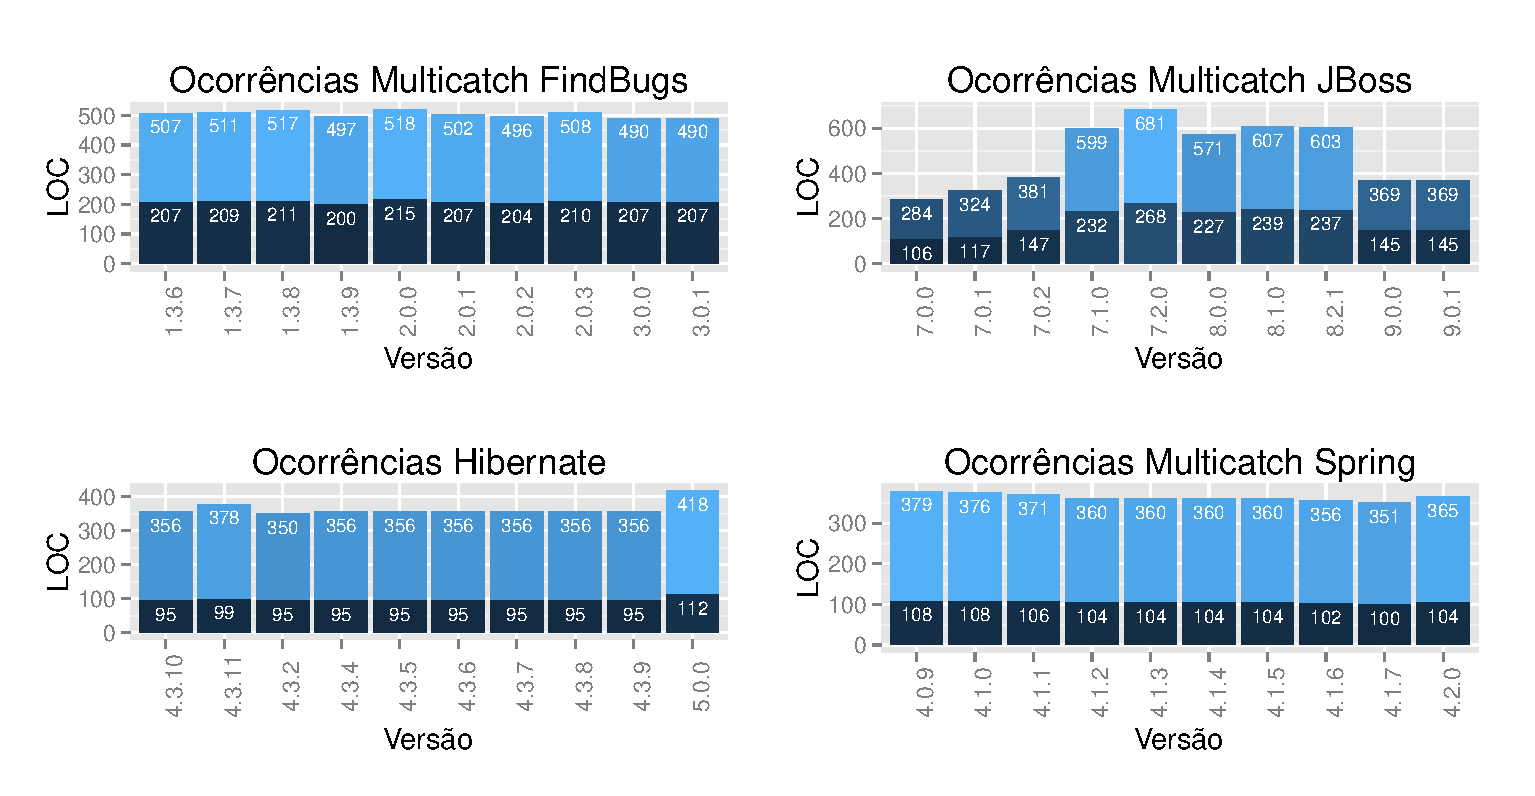
\includegraphics[height=8cm, keepaspectratio]{Imagens/ocorrenciasMulticatchVersoes}
	\label{fig:ocorrenciasMulticatchVersoes}
	\caption{Oportunidades de \textit{Multicatch} nos projetos.}
\end{figure}


%\section{Try Resource}
O visitor responsável por detectar a adoção desta \textit{feature} pesquisou por padrões como o código abaixo onde não foi pesquisado oportunidades de \textit{refactoring} mas sim onde esta característica estava sendo adotada.
\begin{lstlisting}
static String readFirstLineFromFile(String path) throws IOException {
	try (BufferedReader br = new BufferedReader(new FileReader(path))) {
		return br.readLine();
	}
}
\end{lstlisting}

Com o advento do Java 7 foi introduzido o \textit{Try with Resource} onde um \textit{resource} é um objeto que pode ser fechado antes do programa ser encerrado. Com isso promoveu uma maior autonomia e flexibilidade ao programador. Foi encontrado no total 284321 \textit{trys} nos quais  esta \textit{feature} totaliza 1.8\%, ou seja, 5186 casos. Conforme exibido na figura: ~\ref{fig:Try with Resource} exibe a distribuição desta \textit{feature} entre os projetos onde pode-se constatar que somente 4 projetos fizera a adoção. Com exceção do projeto \textit{Jetty} que totaliza 87\% dos casos os demais projetos não aderiram de forma massiva esta caracterísitica.


\begin{figure}[h]
	\center
	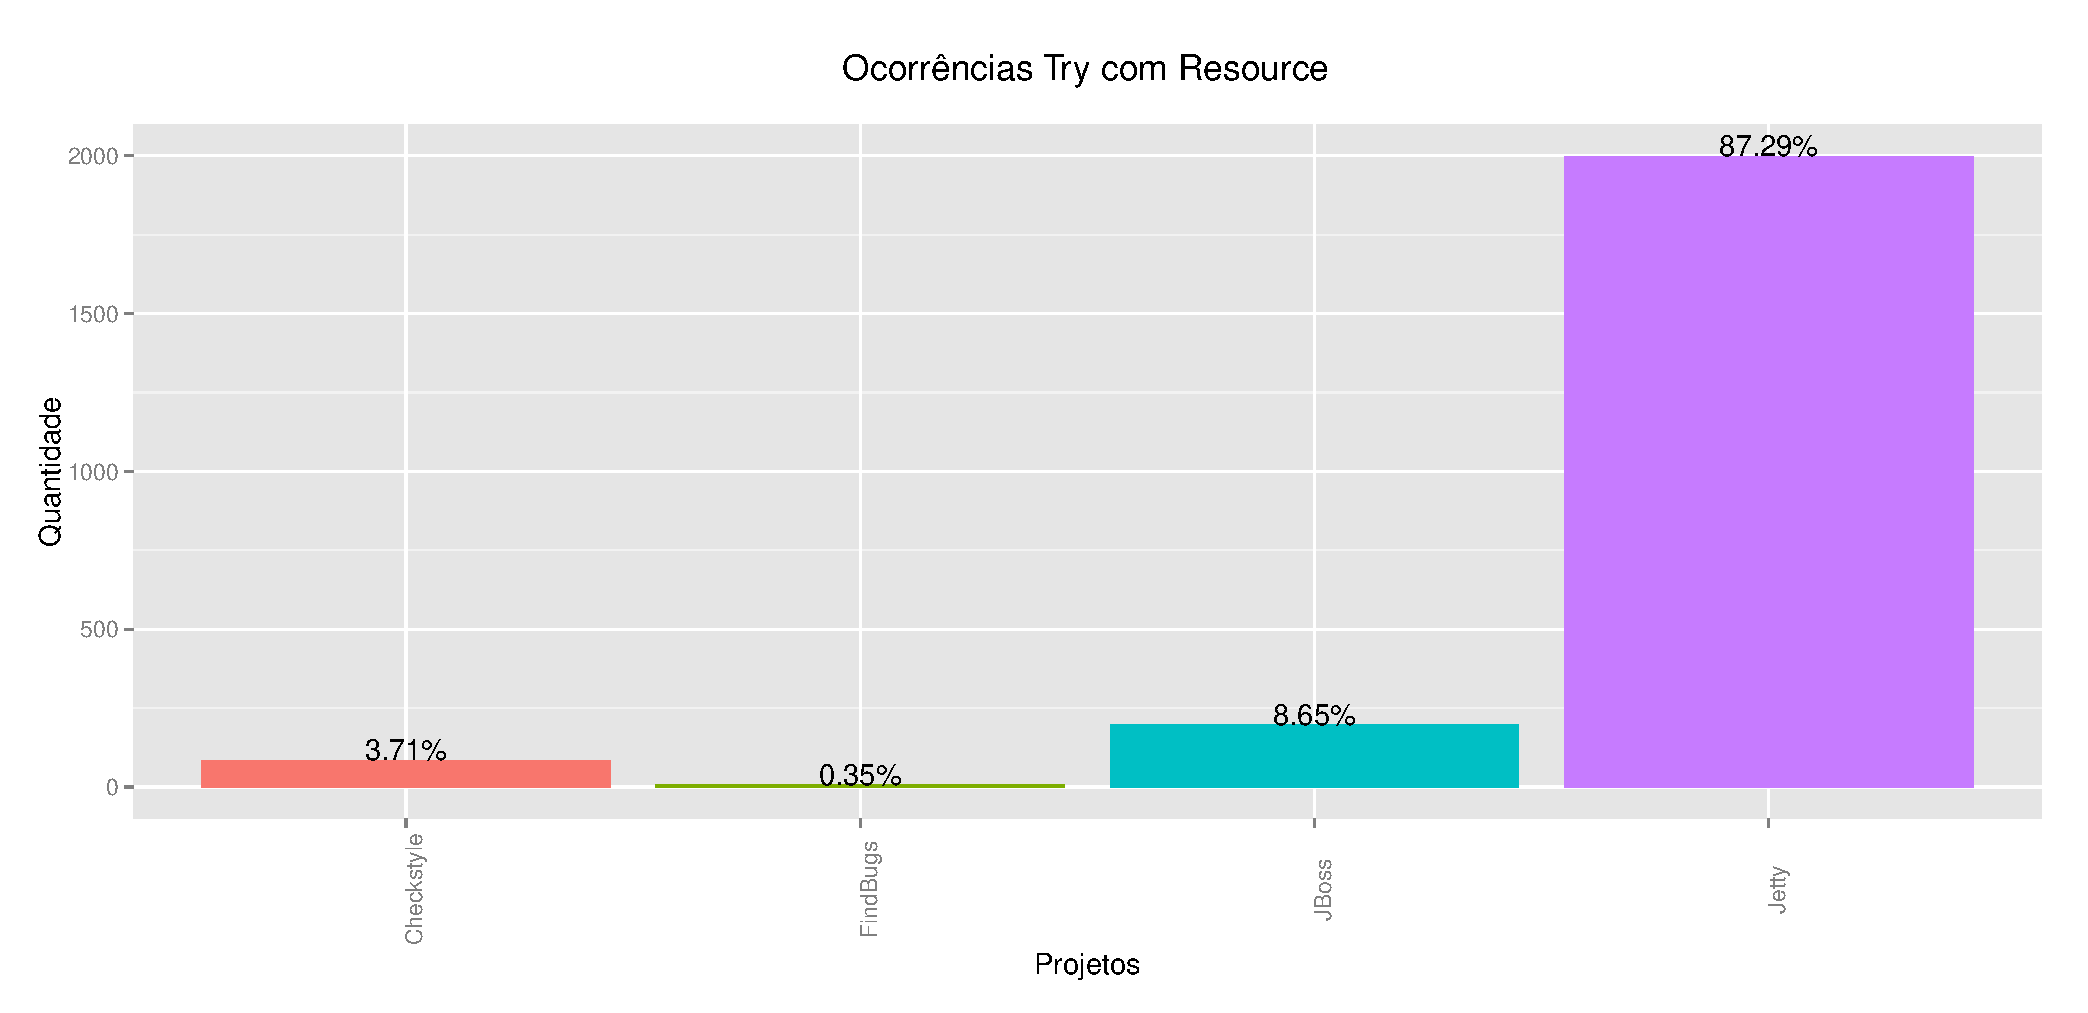
\includegraphics[scale=0.5]{Imagens/ocorrenciasTryResource}
	\label{fig:Try with Resource}
	\caption{Oportunidades de \textit{Try with Resource} nos projetos.}
\end{figure}



%\section{Switch String}
